\documentclass[11pt,a4paper]{article}
\usepackage[T1]{fontenc}
\usepackage[utf8]{inputenc}
\usepackage{lmodern}
\usepackage{textcomp}
\usepackage[left=1.8cm,right=1.8cm,top=2.3cm,bottom=2.2cm,headheight=14pt,headsep=8pt]{geometry}
\usepackage{multicol}
\usepackage{xcolor}
\usepackage{fancyhdr}
\usepackage{graphicx}
\usepackage{array}
\usepackage{amsmath,amssymb}
\usepackage{setspace}
\usepackage{longtable}
\graphicspath{{../}}
\definecolor{ygreen}{RGB}{46,139,87}
\renewcommand{\normalsize}{\fontsize{10.9}{13.4}\selectfont}
\renewcommand{\familydefault}{\rmdefault}
\setlength{\parindent}{0pt}
\setlength{\columnsep}{0.8cm}
\setlength{\columnseprule}{0.4pt}
\setlength{\multicolsep}{3pt plus 1pt minus 1pt}
\renewcommand{\textsubscript}[1]{\ensuremath{_{\text{\fontsize{8}{8}\selectfont #1}}}}
\renewcommand{\textsuperscript}[1]{\ensuremath{^{\text{\fontsize{8}{8}\selectfont #1}}}}
\newcommand{\diqqat}[1]{\par\smallskip\noindent\textbf{Diqqat!} #1\par\medskip}
\newcommand{\javob}{\par\smallskip\noindent\textbf{Javob:} \rule[-2pt]{7.5cm}{0.4pt}\par\smallskip\noindent\textbf{Diqqat!} Javobingizni javoblar varaqasiga ko`chirib yozing.\par\medskip}
\pagestyle{fancy}
\fancyhf{}
\renewcommand{\headrulewidth}{0.4pt}
\fancyhead[L]{\textit{Milliy sertifikat 2026. Kimyo}}
\fancyhead[R]{11-variant}
\fancyfoot[L]{\fontsize{8}{9}\selectfont \textcopyright{} Colba maktabi, 2026}
\fancyfoot[C]{\thepage}
\fancypagestyle{first}{\fancyhf{}\renewcommand{\headrulewidth}{0pt}\fancyfoot[L]{\fontsize{8}{9}\selectfont \textcopyright{} Colba maktabi, 2026}\fancyfoot[C]{\thepage}}
\begin{document}
\normalsize
\thispagestyle{first}
\noindent\fcolorbox{ygreen}{white}{\parbox{\dimexpr\linewidth-2\fboxsep-2\fboxrule\relax}{%
\textbf{\fontsize{13}{15}\selectfont Nazorat testi}\ \textit{\fontsize{10}{12}\selectfont $\cdot$ Aralash test $\cdot$ 11-variant}\hfill
\begin{tabular}[t]{@{}r@{}}\textit{Milliy sertifikat 2026. Kimyo}\\ \textbf{\textit{\fontsize{8}{9}\selectfont Vaqt:}} \textit{\fontsize{10}{12}\selectfont 180 daqiqa}\end{tabular}}}
\par\medskip
\noindent\textit{Davriy jadvaldan foydalanish mumkin.}
\par\medskip
\begin{multicols}{2}
\noindent\textbf{1.} Mo`l kislota bilan Mg ning turli massalari ta'sirlashganda ajralgan H\textsubscript{2} hajmi grafikda keltirilgan (n.sh.).
\begin{center}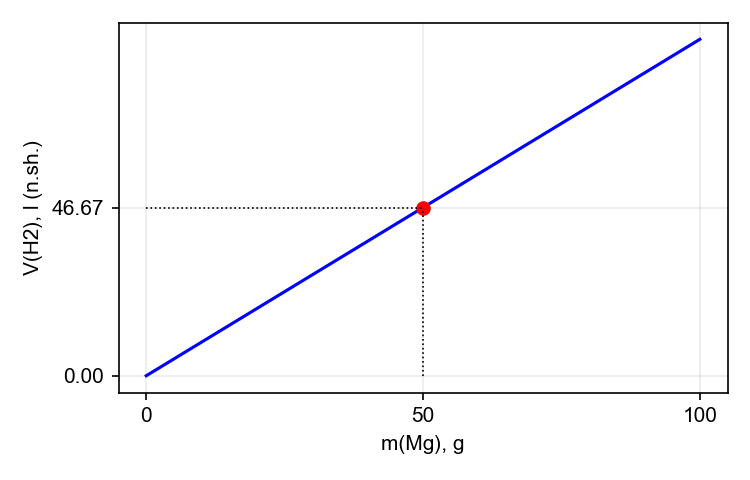
\includegraphics[width=0.86\linewidth]{rasmlar/gen/li_v11_0.png}\end{center}
Mg ning molyar massasini (g/mol) grafikdan \textbf{aniqlang.}

\noindent A)~\textsl{48} \hfill B)~\textsl{12} \hfill C)~\textsl{46,4} \hfill D)~\textsl{24}\par
\vspace{4pt}
\noindent\textbf{2.} Zichligi 1,4 g/ml bo`lgan 30\% li KOH eritmasining molyar \textbf{konsentratsiyasini (mol/l) aniqlang.}

\noindent A)~\textsl{0,75} \hfill B)~\textsl{15} \hfill C)~\textsl{5,36} \hfill D)~\textsl{7,5}\par
\vspace{4pt}
\noindent\textbf{3.} 500 g 12\% li Na\textsubscript{2}SO\textsubscript{4} eritmasidan 80 g suv bug`latildi. Qolgan eritmadagi tuzning massa \textbf{ulushini (\%) toping.}

\noindent A)~\textsl{10,34} \hfill B)~\textsl{1,92} \hfill C)~\textsl{14,29} \hfill D)~\textsl{11,43}\par
\vspace{4pt}
\noindent\textbf{4.} Jadvalda bog`lar hosil qiluvchi atomlarning elektrmanfiyliklari berilgan:
\begin{center}
\renewcommand{\arraystretch}{1.15}
\begin{tabular}{|c|c|c|}\hline
\textbf{Bog`} & \textbf{EM (1-atom)} & \textbf{EM (2-atom)} \\ \hline
H--Cl & 2,1 & 3 \\ \hline
Mg--O & 1,2 & 3,5 \\ \hline
C--H & 2,5 & 2,1 \\ \hline
Al--Cl & 1,5 & 3 \\ \hline
\end{tabular}
\end{center}
Qaysi bog` eng qutbli (eng ko`p ionli xarakterga ega)?

\noindent A)~\textsl{H--Cl} \hfill B)~\textsl{C--H} \hfill C)~\textsl{Mg--O} \hfill D)~\textsl{Al--Cl}\par
\vspace{4pt}
\noindent\textbf{5.} 1 mol NH\textsubscript{3} tarkibida necha mol atom bor?

\noindent A)~\textsl{3} \hfill B)~\textsl{5} \hfill C)~\textsl{4} \hfill D)~\textsl{1}\par
\vspace{4pt}
\noindent\textbf{6.} Na\textsubscript{2}CO\textsubscript{3}$\cdot$10H\textsubscript{2}O kristallogidratida kristallizatsion suvning massa \textbf{ulushini (\%) aniqlang.}

\noindent A)~\textsl{62,9} \hfill B)~\textsl{37,1} \hfill C)~\textsl{31,5} \hfill D)~\textsl{169,8}\par
\vspace{4pt}
\noindent\textbf{7.} K\textsubscript{2}CO\textsubscript{3} ning suvli eritmasi inert elektrodlar bilan elektroliz qilinganda qaysi moddalar ajraladi?

\noindent\begin{tabular}{@{}p{0.47\linewidth}@{}p{0.47\linewidth}@{}}
A)~\textsl{Ag va O\textsubscript{2}} & B)~\textsl{H\textsubscript{2} va O\textsubscript{2}} \\
C)~\textsl{Zn, H\textsubscript{2} va O\textsubscript{2}} & D)~\textsl{Cu va O\textsubscript{2}} \\
\end{tabular}\par
\vspace{4pt}
\noindent\textbf{8.} Jadvalda nuklidlarning proton soni (\textit{Z}) va massa soni (A) berilgan:
\begin{center}
\renewcommand{\arraystretch}{1.15}
\begin{tabular}{|c|c|c|}\hline
\textbf{Nuklid} & \textbf{\textit{Z}} & \textbf{A} \\ \hline
\textit{X} & 17 & 35 \\ \hline
\textit{Y} & 17 & 36 \\ \hline
T & 18 & 35 \\ \hline
\textit{U} & 18 & 36 \\ \hline
\textit{V} & 17 & 36 \\ \hline
\end{tabular}
\end{center}
\textit{X} nuklidning nechta izotopi jadvalda keltirilgan?

\noindent A)~\textsl{3} \hfill B)~\textsl{4} \hfill C)~\textsl{1} \hfill D)~\textsl{2}\par
\vspace{4pt}
\noindent\textbf{9.} Quyidagi tuzlarning qaysilari suvli eritmasi ishqoriy muhitga ega? 1) KNO\textsubscript{3}; 2) NH\textsubscript{4}Cl; 3) Na\textsubscript{2}SO\textsubscript{4}; 4) CH\textsubscript{3}COONa

\noindent A)~\textsl{4} \hfill B)~\textsl{2, 3} \hfill C)~\textsl{1, 2} \hfill D)~\textsl{1, 4}\par
\vspace{4pt}
\noindent\textbf{10.} H\textsubscript{2}N--CH\textsubscript{2}--COOH molekulasida sp\textsuperscript{2} gibridlangan uglerod atomlari nechta?

\noindent A)~\textsl{2} \hfill B)~\textsl{1} \hfill C)~\textsl{3} \hfill D)~\textsl{4}\par
\vspace{4pt}
\noindent\textbf{11.} 2SO\textsubscript{2} + O\textsubscript{2} $\rightleftarrows$ 2SO\textsubscript{3} + Q muvozanatni o`ngga siljitadigan \textbf{o`zgarishlarni toping}: 1) katalizator qo`shish; 2) bosimni oshirish; 3) bosimni pasaytirish; 4) haroratni oshirish.

\noindent A)~\textsl{4} \hfill B)~\textsl{2} \hfill C)~\textsl{2, 3} \hfill D)~\textsl{3, 4}\par
\vspace{4pt}
\noindent\textbf{12.} Mishyak atomining p- va d- pog`onachalaridagi elektronlardan nechtasining magnit kvant soni m\_l = 1 ga teng? (\textit{Z} = 33)

\noindent A)~\textsl{7} \hfill B)~\textsl{8} \hfill C)~\textsl{6} \hfill D)~\textsl{9}\par
\vspace{4pt}
\noindent\textbf{13.} Quyidagilarni jism va moddalarga ajrating: suv, mis, mixga, stakan, alyuminiy, tanga. Ulardan nechtasi modda?

\noindent A)~\textsl{3} \hfill B)~\textsl{4} \hfill C)~\textsl{2} \hfill D)~\textsl{5}\par
\vspace{4pt}
\noindent\textbf{14.} Nodir gazlar haqida qaysi fikrlar to`g`ri? 1) Geliy eng yengil inert gaz; 2) Argon elektr lampalarida ishlatiladi; 3) Neon atomida 8 ta tashqi elektron bor; 4) Neon reklama naylarida ishlatiladi

\noindent\begin{tabular}{@{}p{0.47\linewidth}@{}p{0.47\linewidth}@{}}
A)~\textsl{1, 3, 4} & B)~\textsl{1, 2, 4} \\
C)~\textsl{1, 2, 3, 4} & D)~\textsl{1, 2, 3} \\
\end{tabular}\par
\vspace{4pt}
\noindent\textbf{15.} KNO\textsubscript{3} qizdirilganda qanday moddalar hosil bo`ladi?

\noindent\begin{tabular}{@{}p{0.47\linewidth}@{}p{0.47\linewidth}@{}}
A)~\textsl{KNO\textsubscript{2} va O\textsubscript{2}} & B)~\textsl{CuO, NO\textsubscript{2} va O\textsubscript{2}} \\
C)~\textsl{ZnO, NO\textsubscript{2} va O\textsubscript{2}} & D)~\textsl{N\textsubscript{2}O va H\textsubscript{2}O} \\
\end{tabular}\par
\vspace{4pt}
\noindent\textbf{16.} Qaysi juftliklar o`zaro reaksiyaga kirishadi? 1) Zn va NaOH; 2) Fe\textsubscript{2}O\textsubscript{3} va H\textsubscript{2}O; 3) MgCl\textsubscript{2} va KNO\textsubscript{3}; 4) Al\textsubscript{2}O\textsubscript{3} va NaOH

\noindent A)~\textsl{1} \hfill B)~\textsl{1, 4} \hfill C)~\textsl{1, 2, 3} \hfill D)~\textsl{1, 3, 4}\par
\vspace{4pt}
\noindent\textbf{17.} 17 g NaNO\textsubscript{3} to`liq parchalanguncha qizdirildi. Qattiq qoldiq \textbf{massasini (g) aniqlang.}

\noindent A)~\textsl{17} \hfill B)~\textsl{27,6} \hfill C)~\textsl{6,9} \hfill D)~\textsl{13,8}\par
\vspace{4pt}
\noindent\textbf{18.} 6,2 g fosfor yondirilib, hosil bo`lgan oksid suvda eritildi (ortofosfat kislota), so`ng 0,3 mol NaOH qo`shildi. Hosil bo`lgan NaH\textsubscript{2}PO\textsubscript{4} \textbf{massasini (g) aniqlang.}

\noindent A)~\textsl{12} \hfill B)~\textsl{24} \hfill C)~\textsl{6} \hfill D)~\textsl{32,8}\par
\vspace{4pt}
\noindent\textbf{19.} Cl\textsubscript{2} + 2NaOH $\to$ NaCl + NaClO + H\textsubscript{2}O reaksiyasida 4,48 l (n.sh.) Cl\textsubscript{2} ishtirok etdi (unum 60\%). NaClO \textbf{massasini (g) toping.}

\noindent A)~\textsl{14,9} \hfill B)~\textsl{8,94} \hfill C)~\textsl{17,88} \hfill D)~\textsl{4,47}\par
\vspace{4pt}
\noindent\textbf{20.} Reaksiya tenglamasi: C\textsubscript{3}H\textsubscript{8} + 5O\textsubscript{2} $\to$ 3CO\textsubscript{2} + 4H\textsubscript{2}O. Reaksiyaga 11,2 l (n.sh.) C\textsubscript{3}H\textsubscript{8} kirishdi (unum 50\%). O\textsubscript{2} \textbf{hajmini (l, n.sh.) hisoblang.}

\noindent A)~\textsl{28} \hfill B)~\textsl{2,24} \hfill C)~\textsl{56} \hfill D)~\textsl{14}\par
\vspace{4pt}
\noindent\textbf{21.} C\textsubscript{2}H\textsubscript{5}OH $\to$ C\textsubscript{2}H\textsubscript{4} + H\textsubscript{2}O jarayoni uchun 46 g C\textsubscript{2}H\textsubscript{5}OH olingan. C\textsubscript{2}H\textsubscript{4} \textbf{hajmini (l, n.sh.) aniqlang.}

\noindent A)~\textsl{44,8} \hfill B)~\textsl{22,4} \hfill C)~\textsl{11,2} \hfill D)~\textsl{33,6}\par
\vspace{4pt}
\noindent\textbf{22.} 32 g CaC\textsubscript{2} suv bilan reaksiyaga kirishganda ajraladigan asetilen \textbf{hajmini (l, n.sh.) aniqlang} (unum 80\%).

\noindent A)~\textsl{11,2} \hfill B)~\textsl{8,96} \hfill C)~\textsl{25,6} \hfill D)~\textsl{22,4}\par
\vspace{4pt}
\noindent\textbf{23.} C\textsubscript{6}H\textsubscript{5}NO\textsubscript{2} + H\textsubscript{2} (kat.) reaksiyasi natijasida qaysi organik modda hosil bo`ladi?

\noindent\begin{tabular}{@{}p{0.47\linewidth}@{}p{0.47\linewidth}@{}}
A)~\textsl{etanol} & B)~\textsl{etilatsetat} \\
C)~\textsl{benzol} & D)~\textsl{anilin} \\
\end{tabular}\par
\vspace{4pt}
\noindent\textbf{24.} 44 g CH\textsubscript{3}CHO dan quyidagi ikki bosqichda CH\textsubscript{3}COONa olinadi: 1) CH\textsubscript{3}CHO + 2Ag\textsubscript{2}O $\to$ CH\textsubscript{3}COOH + 4Ag (unum 60\%); 2) CH\textsubscript{3}COOH + NaHCO\textsubscript{3} $\to$ CH\textsubscript{3}COONa + CO\textsubscript{2} + H\textsubscript{2}O (unum 90\%). Oxirgi mahsulot CH\textsubscript{3}COONa ning \textbf{massasini (g) toping.}

\noindent A)~\textsl{73,8} \hfill B)~\textsl{49,2} \hfill C)~\textsl{44,28} \hfill D)~\textsl{82}\par
\vspace{4pt}
\noindent\textbf{25.} Karbon kislotalar haqida qaysi fikrlar to`g`ri? 1) Karboksil guruh karbonil va gidroksil guruhlardan iborat; 2) Qattiq suvda sovun yaxshi ko`piklanadi; 3) Olein kislota Br\textsubscript{2} ni biriktiradi; 4) Sirka angidrid ikki molekula sirka kislotadan suv chiqib hosil bo`ladi

\noindent A)~\textsl{1, 2, 3} \hfill B)~\textsl{1, 3, 4} \hfill C)~\textsl{1, 3} \hfill D)~\textsl{2, 4}\par
\vspace{4pt}
\noindent\textbf{26.} 89 g tristearin gidrolizlanganda necha gramm glitserin hosil bo`ladi?

\noindent A)~\textsl{27,6} \hfill B)~\textsl{4,6} \hfill C)~\textsl{89} \hfill D)~\textsl{9,2}\par
\vspace{4pt}
\noindent\textbf{27.} Rasmda ko`rsatilgan molekulalar H\textsubscript{2}SO\textsubscript{4} ishtirokida o`zaro reaksiyaga kirishdi. Hosil bo`lgan organik moddaning \textbf{nomini toping.}
\begin{center}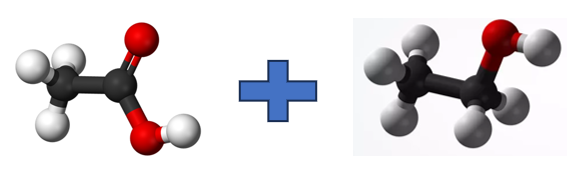
\includegraphics[width=0.86\linewidth]{rasmlar/m_efir.png}\end{center}

\noindent\begin{tabular}{@{}p{0.47\linewidth}@{}p{0.47\linewidth}@{}}
A)~\textsl{etilatsetat} & B)~\textsl{metilatsetat} \\
C)~\textsl{etilformiat} & D)~\textsl{propil spirti} \\
\end{tabular}\par
\vspace{4pt}
\noindent\textbf{28.} Aminlar, aminokislotalar va oqsillar haqida qaysi fikrlar to`g`ri? 1) Nitrobenzoldan anilin Zinin reaksiyasi bilan olinadi; 2) Dipeptidda 2 ta peptid bog` bor; 3) Anilin bromli suv bilan oq cho`kma beradi; 4) Aminlar kuchsiz asoslar xossasini namoyon qiladi

\noindent A)~\textsl{3, 4} \hfill B)~\textsl{2, 3, 4} \hfill C)~\textsl{2, 4} \hfill D)~\textsl{1, 3, 4}\par
\vspace{4pt}
\noindent\textbf{29.} Yuqori molekulyar birikmalar haqida qaysi fikrlar to`g`ri? 1) Teflon --- polivinilxlorid; 2) Termoreaktiv polimerlar qizdirilganda qayta yumshaydi; 3) Fenolformaldegid smola polikondensatsiya mahsuloti; 4) Polimerning M = zveno M $\cdot$ polimerlanish darajasi

\noindent A)~\textsl{1, 4} \hfill B)~\textsl{1, 2} \hfill C)~\textsl{3, 4} \hfill D)~\textsl{2, 4}\par
\vspace{4pt}
\noindent\textbf{30.} 40\% li va 5\% li eritmalardan 200 g 35\% li eritma tayyorlash uchun 40\% li eritmadan necha gramm olish kerak?

\noindent A)~\textsl{28,57} \hfill B)~\textsl{175} \hfill C)~\textsl{342,86} \hfill D)~\textsl{171,43}\par
\vspace{4pt}
\noindent\textbf{31.} 300 g 15\% li MgSO\textsubscript{4} eritmasiga 10 g shu tuzning o`zi qo`shilib eritildi. Hosil bo`lgan eritmaning massa \textbf{ulushini (\%) aniqlang.}

\noindent A)~\textsl{18,33} \hfill B)~\textsl{9,17} \hfill C)~\textsl{17,74} \hfill D)~\textsl{14,19}\par
\vspace{4pt}
\noindent\textbf{32.} Rasmdagi asbobda 9,2 g etanol konsentrlangan H\textsubscript{2}SO\textsubscript{4} bilan 170 \textdegree{}C da qizdirilib, 80\% unum bilan etilen olindi. Hosil bo`lgan etilen \textbf{hajmini (l, n.sh.) aniqlang.}
\begin{center}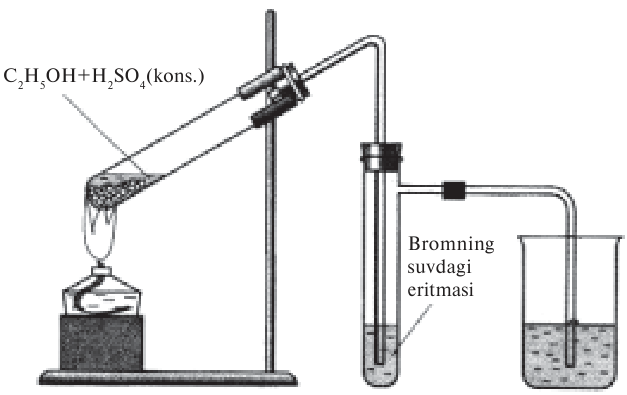
\includegraphics[width=0.86\linewidth]{rasmlar/darslik/d_etilen.png}\end{center}

\noindent\begin{tabular}{@{}p{0.47\linewidth}@{}p{0.47\linewidth}@{}}
A)~\textsl{4,48} & B)~\textsl{7,17} \\
C)~\textsl{3,58} & D)~\textsl{1,79   ---} \\
\end{tabular}\par
\vspace{4pt}
\end{multicols}
\medskip
\noindent\setlength{\fboxsep}{0pt}\fbox{\begin{tabular}{p{0.74\linewidth}|p{0.2\linewidth}}
\parbox[t]{0.72\linewidth}{\vspace{3pt}\textbf{Topshiriqlar (33--35) va javob variant (A--F)larini o`zaro to`g`ri moslashtiring.} KCl va KI dan iborat 24,05 g aralashma suvda eritilib, mo`l AgNO\textsubscript{3} eritmasi qo`shildi; hosil bo`lgan cho`kmalarning umumiy massasi 37,85 g.
\vspace{3pt}} & \parbox[t]{0.19\linewidth}{\vspace{3pt}A~\textsl{20,2}\\[3pt]
B~\textsl{7,45}\\[3pt]
C~\textsl{340}\\[3pt]
D~\textsl{10,1}\\[3pt]
E~\textsl{3,73}\\[3pt]
F~\textsl{5,96}}\\ \hline
\parbox[t]{0.72\linewidth}{\vspace{2pt}\textbf{33. Aralashmadagi KCl massasini (g) aniqlang.}\vspace{2pt}} & \\ \hline
\parbox[t]{0.72\linewidth}{\vspace{2pt}\textbf{34. Sarflangan 10\% li AgNO\textsubscript{3} eritmasining massasini (g) aniqlang (M(AgNO\textsubscript{3}) = 170 g/mol).}\vspace{2pt}} & \\ \hline
\parbox[t]{0.72\linewidth}{\vspace{2pt}\textbf{35. Eritmada hosil bo`lgan nitratlarning umumiy massasini (g) aniqlang.}\vspace{2pt}} & 
\end{tabular}}
\par\bigskip
\noindent\textbf{36.} K\textsubscript{2}Cr\textsubscript{2}O\textsubscript{7} + FeSO\textsubscript{4} + H\textsubscript{2}SO\textsubscript{4} $\to$ Cr\textsubscript{2}(SO\textsubscript{4})\textsubscript{3} + Fe\textsubscript{2}(SO\textsubscript{4})\textsubscript{3} + K\textsubscript{2}SO\textsubscript{4} + H\textsubscript{2}O reaksiya tenglamasini tenglang va barcha koeffitsiyentlar \textbf{yig`indisini aniqlang.}
\javob
\noindent\textbf{37.} CuSO\textsubscript{4} eritmasi inert elektrodlar yordamida 5 A tok kuchi bilan 965 s elektroliz qilindi. Katodda ajralgan Cu massasi (g) \textbf{ni toping.}
\javob
\noindent\textbf{38.} 37,6 g Cu(NO\textsubscript{3})\textsubscript{2} qizdirilganda qisman parchalandi, qattiq qoldiq massasi 26,8 g bo`ldi. Ajralgan gazlar (n.sh.) \textbf{hajmini (l) hisoblang.}
\javob
\noindent\textbf{39.} 9,2 g etanol avval sirka aldegidgacha (unum 90\%), so`ng sirka kislotagacha (unum 75\%) oksidlandi; hosil bo`lgan kislota mo`l etanol bilan efirlandi (unum 100\%). Etilatsetat \textbf{massasini (g) toping.}
\javob
\noindent\textbf{40.} Polimerlanish darajasi 500 bo`lgan polivinilxlorid ning 31,25 g namunasini olish uchun polimerlanish unumi 50\% bo`lganda qancha monomer (C\textsubscript{2}H\textsubscript{3}Cl) kerak (g)?
\javob
\par\bigskip\begin{center}\textbf{\fontsize{13}{15}\selectfont YOZMA ISH}\end{center}
\noindent\textbf{41.} \textbf{Topshiriqni bajarish jarayonida barcha reaksiya tenglamalarini yozing. Miqdoriy va arifmetik hisoblashlarni (unga asos bo`lgan usul yoki formulani ko`rsatgan holda) uzviy ketma-ketlikda bajaring.}\par\smallskip
Tarkibida 2 mol H\textsubscript{2}SO\textsubscript{4} va 1 mol SO\textsubscript{3} bo`lgan oleum namunasi 500 g suvda eritildi.\par
\noindent 1)Oleumdagi SO\textsubscript{3} ning massa ulushini (\%) hisoblang.\par
\noindent 2)SO\textsubscript{3} suv bilan reaksiyaga kirishgandan so`ng eritmadagi H\textsubscript{2}SO\textsubscript{4} ning umumiy miqdorini (mol) toping (reaksiya tenglamasini yozing). Hosil bo`lgan eritmadagi suvning massasini (g) ham hisoblang.\par
\noindent 3)Hosil bo`lgan eritmadagi H\textsubscript{2}SO\textsubscript{4} ning massa ulushini (\%) aniqlang.\par
\noindent 4)Shu eritmani to`liq neytrallash uchun zichligi 1,11 g/ml bo`lgan 10\% li NaOH eritmasidan necha ml kerak? Hosil bo`lgan Na\textsubscript{2}SO\textsubscript{4} massasini (g) ham toping.\par
\noindent 5)Eritmaga mo`l BaCl\textsubscript{2} eritmasi qo`shilganda hosil bo`ladigan cho`kma massasini (g) toping. Hosil bo`lgan eritmaning zichligi 1,4 g/ml bo`lsa, uning molyar konsentratsiyasini (mol/l) toping.\par
\diqqat{Mazkur topshiriq kengaytirilgan javobni talab etib, uning yechilish usuli va shu usul asosidagi barcha hisoblash amallari javoblar varaqasida aks etishi lozim.}
\noindent\textbf{42.} Quyidagi o`zgarishlar zanjirida \textit{X}, \textit{Y}, \textit{Z} noma'lum organik moddalar:\par
\[\setlength{\fboxsep}{0pt}\text{CH\textsubscript{3}Cl}\xrightarrow{\text{Na}}\text{\textit{X}}\xrightarrow{\text{Cl\textsubscript{2}, yorug`lik}}\text{\textit{Y}}\xrightarrow{\text{KOH (suvli)}}\text{\textit{Z}}\xrightarrow{\text{Na}}\text{C\textsubscript{2}H\textsubscript{5}ONa}\]
\noindent 1)CH\textsubscript{3}Cl $\to$ \textit{X} : reaksiya tenglamasini yozing; hosil bo`lgan moddani nomlang.\par
\noindent 2)\textit{X} $\to$ \textit{Y} : reaksiya tenglamasini yozing; hosil bo`lgan moddani nomlang.\par
\noindent 3)\textit{Y} $\to$ \textit{Z} : reaksiya tenglamasini yozing; hosil bo`lgan moddani nomlang.\par
\noindent 4)\textit{Z} $\to$ C\textsubscript{2}H\textsubscript{5}ONa : reaksiya tenglamasini yozing; hosil bo`lgan moddani nomlang.\par
\diqqat{Mazkur topshiriq kengaytirilgan javobni talab etib, uning yechilish usuli va shu usul asosidagi barcha hisoblash amallari javoblar varaqasida aks etishi lozim.}
\noindent\textbf{43.} \textbf{Topshiriqni bajarish jarayonida barcha reaksiya tenglamalarini yozing. Miqdoriy va arifmetik hisoblashlarni (unga asos bo`lgan usul yoki formulani ko`rsatgan holda) uzviy ketma-ketlikda bajaring.}\par\smallskip
0,2 mol AlCl\textsubscript{3} saqlagan eritmaga NaOH eritmasi qo`shildi. Avval 0,6 mol NaOH qo`shilganda cho`kma hosil bo`ldi, so`ng yana 0,2 mol NaOH qo`shilganda cho`kma to`liq erib ketdi (Na[Al(OH)\textsubscript{4}] hosil bo`ldi).\par
\noindent 1)Cho`kma hosil bo`lish va erish reaksiyalari tenglamalarini yozing. Cho`kma massasini (g) hisoblang.\par
\noindent 2)Jami sarflangan NaOH massasini (g) aniqlang.\par
\noindent 3)Hosil bo`lgan Na[Al(OH)\textsubscript{4}] eritmasidan mo`l CO\textsubscript{2} o`tkazilganda cho`kadigan Al(OH)\textsubscript{3} massasini (g) toping.\par
\noindent 4)Al(OH)\textsubscript{3} cho`kmasi qizdirilganda hosil bo`ladigan oksid massasini (g) hisoblang.\par
\noindent 5)Na[Al(OH)\textsubscript{4}] eritmasining hajmi 500 ml bo`lsa, tuzning molyar konsentratsiyasini (mol/l) hisoblang.\par
\diqqat{Mazkur topshiriq kengaytirilgan javobni talab etib, uning yechilish usuli va shu usul asosidagi barcha hisoblash amallari javoblar varaqasida aks etishi lozim.}
\newpage
\noindent\textbf{\fontsize{13}{15}\selectfont Nazorat testi}\ \textit{$\cdot$ 11-variant}\hfill \textbf{Javoblar kaliti}\par\smallskip\hrule\smallskip
\textit{Faqat o`qituvchi uchun.}\par\medskip
\noindent\textbf{1--32-savollar}\par\smallskip
\noindent\begin{tabular}{|c|c|c|c|c|c|c|c|c|c|c|c|c|c|c|c|}\hline
\textbf{1} & \textbf{2} & \textbf{3} & \textbf{4} & \textbf{5} & \textbf{6} & \textbf{7} & \textbf{8} & \textbf{9} & \textbf{10} & \textbf{11} & \textbf{12} & \textbf{13} & \textbf{14} & \textbf{15} & \textbf{16}\\\hline
\textsl{D} & \textsl{D} & \textsl{C} & \textsl{C} & \textsl{C} & \textsl{A} & \textsl{B} & \textsl{D} & \textsl{A} & \textsl{B} & \textsl{B} & \textsl{A} & \textsl{A} & \textsl{C} & \textsl{A} & \textsl{B}\\\hline
\textbf{17} & \textbf{18} & \textbf{19} & \textbf{20} & \textbf{21} & \textbf{22} & \textbf{23} & \textbf{24} & \textbf{25} & \textbf{26} & \textbf{27} & \textbf{28} & \textbf{29} & \textbf{30} & \textbf{31} & \textbf{32}\\\hline
\textsl{D} & \textsl{A} & \textsl{B} & \textsl{A} & \textsl{B} & \textsl{B} & \textsl{D} & \textsl{C} & \textsl{B} & \textsl{D} & \textsl{A} & \textsl{D} & \textsl{C} & \textsl{D} & \textsl{C} & \textsl{C}\\\hline
\end{tabular}\par\medskip
\noindent\textbf{33--35-savollar}\par\smallskip
\noindent\begin{tabular}{|c|c|c|}\hline \textbf{No} & \textbf{Javob} & \textbf{Qiymat}\\\hline
33 & \textsl{B} & 7,45\\\hline
34 & \textsl{C} & 340\\\hline
35 & \textsl{A} & 20,2\\\hline
\end{tabular}\par\medskip
\noindent\textbf{36--40-savollar}\par\smallskip
\noindent\begin{tabular}{|c|c|}\hline \textbf{No} & \textbf{To`g`ri javob}\\\hline
36 & 26\\\hline
37 & 1,6\\\hline
38 & 5,6\\\hline
39 & 11,88\\\hline
40 & 62,5\\\hline
\end{tabular}\par\medskip
\noindent\textbf{41--43-topshiriqlar: qisqa yechim}\par\smallskip
\noindent\textbf{41-topshiriq.}\par
\noindent 1) m(oleum) = 2$\cdot$98 + 1$\cdot$80 = 276 g; $\omega$(SO\textsubscript{3}) = 80/276 = \textbf{28,99\%}\par
\noindent 2) SO\textsubscript{3} + H\textsubscript{2}O $\to$ H\textsubscript{2}SO\textsubscript{4}: n = 2 + 1 = \textbf{3 mol}; m(H\textsubscript{2}O) = 500 $-$ 18$\cdot$1 = \textbf{482 g}\par
\noindent 3) m(H\textsubscript{2}SO\textsubscript{4}) = 3$\cdot$98 = 294 g; m(eritma) = 276 + 500 = 776 g $\to$ \textbf{37,89\%}\par
\noindent 4) H\textsubscript{2}SO\textsubscript{4} + 2NaOH $\to$ Na\textsubscript{2}SO\textsubscript{4} + 2H\textsubscript{2}O: m(NaOH) = 240 g; eritma 2400 g; \textit{V} = 2400/1,11 = \textbf{2162,2 ml}; m(Na\textsubscript{2}SO\textsubscript{4}) = 3$\cdot$142 = \textbf{426 g}\par
\noindent 5) H\textsubscript{2}SO\textsubscript{4} + BaCl\textsubscript{2} $\to$ BaSO\textsubscript{4}$\downarrow$ + 2HCl: 3$\cdot$233 = \textbf{699 g}; C = 10$\cdot$$\omega$$\cdot$$\rho$/M = 10$\cdot$37,89$\cdot$1,4/98 = \textbf{5,41 mol/l}\par
\noindent Jami: M 15 + A 10 = 25 ball.\par
\noindent\textbf{42-topshiriq.}\par
\noindent 1) CH\textsubscript{3}Cl + Na $\to$ C\textsubscript{2}H\textsubscript{6} (etan)\par
\noindent 2) C\textsubscript{2}H\textsubscript{6} + Cl\textsubscript{2}, yorug`lik $\to$ C\textsubscript{2}H\textsubscript{5}Cl (xloretan)\par
\noindent 3) C\textsubscript{2}H\textsubscript{5}Cl + KOH (suvli) $\to$ C\textsubscript{2}H\textsubscript{5}OH (etanol)\par
\noindent 4) C\textsubscript{2}H\textsubscript{5}OH + Na $\to$ C\textsubscript{2}H\textsubscript{5}ONa (natriy etilat)\par
\noindent Jami 25 ball.\par
\noindent\textbf{43-topshiriq.}\par
\noindent 1) AlCl\textsubscript{3} + 3NaOH $\to$ Al(OH)\textsubscript{3}$\downarrow$ + 3NaCl; Al(OH)\textsubscript{3} + NaOH $\to$ Na[Al(OH)\textsubscript{4}]; n(Al(OH)\textsubscript{3}) = 0,2 mol $\to$ \textbf{15,6 g}\par
\noindent 2) n(NaOH) = 0,6 + 0,2 = 0,8 mol $\to$ \textbf{32 g}\par
\noindent 3) Na[Al(OH)\textsubscript{4}] + CO\textsubscript{2} $\to$ Al(OH)\textsubscript{3}$\downarrow$ + NaHCO\textsubscript{3}: \textbf{15,6 g}\par
\noindent 4) 2Al(OH)\textsubscript{3} $\to$ Al\textsubscript{2}O\textsubscript{3} + 3H\textsubscript{2}O: n(Al\textsubscript{2}O\textsubscript{3}) = 0,1 mol $\to$ \textbf{10,2 g}\par
\noindent 5) C = 0,2/0,5 = \textbf{0,4 mol/l}\par
\noindent Jami: M 15 + A 10 = 25 ball.\par
\par\bigskip\noindent\textbf{Mavzular taqsimoti}\par\smallskip
{\small\noindent\begin{longtable}{|c|p{7.2cm}|p{5.4cm}|c|}\hline \textbf{No} & \textbf{Mavzu} & \textbf{Tekshiriladigan ko`nikma} & \textbf{Ball}\\\hline
1 & 8-sinf (molyar hajm, grafik) & Grafik tahlili & 1\\\hline
2 & 11-sinf 4-bob (molyar konsentratsiya) & Hisoblash va masala yechish & 1\\\hline
3 & Tirkashev III bob (eritmalar) & Hisoblash va masala yechish & 1\\\hline
4 & 8-sinf (kimyoviy bog`lanish turlari, jadval) & Jadval tahlili & 1\\\hline
5 & 7-sinf (mol) & Hisoblash va masala yechish & 1\\\hline
6 & 7-sinf; Tirkashev (kristallogidrat) & Hisoblash va masala yechish & 1\\\hline
7 & 11-sinf 8-bob; Tirkashev \textit{V} bob (elektroliz) & Bilim va tushunish & 1\\\hline
8 & 8-sinf (izotoplar, izobarlar, jadval) & Jadval tahlili & 1\\\hline
9 & 9-sinf (gidroliz); Tirkashev IV bob & Bilim va tushunish & 1\\\hline
10 & 10-sinf \S{}17 & Bilim va tushunish & 1\\\hline
11 & Tirkashev VI bob (Le-Shatelye) & Bilim va tushunish & 1\\\hline
12 & Tirkashev I bob (kvant sonlari) & Bilim va tushunish & 1\\\hline
13 & 7-sinf (jism va modda) & Bilim va tushunish & 1\\\hline
14 & Tashev (nodir gazlar); 8-sinf & Bilim va tushunish & 1\\\hline
15 & Tashev (nitratlar) & Bilim va tushunish & 1\\\hline
16 & 9-sinf; Tashev (anorganik birikmalar xossalari) & Bilim va tushunish & 1\\\hline
17 & Tashev (nitratlar termik parchalanishi) & Hisoblash va masala yechish & 1\\\hline
18 & Tashev (fosfor) & Hisoblash va masala yechish & 1\\\hline
19 & 9-sinf; Tirkashev (galogenlar, hisob) & Hisoblash va masala yechish & 1\\\hline
20 & 10-sinf (alkan, hisob) & Hisoblash va masala yechish & 1\\\hline
21 & 10-sinf (alken, hisob) & Hisoblash va masala yechish & 1\\\hline
22 & 10-sinf \S{}15 (asetilen olinishi) & Hisoblash va masala yechish & 1\\\hline
23 & 10-sinf (olinish usullari) & Bilim va tushunish & 1\\\hline
24 & 10-sinf (ikki bosqichli hisob) & Hisoblash va masala yechish & 1\\\hline
25 & 10-sinf (mavzuga oid paragraflar); Abdusamatov & Bilim va tushunish & 1\\\hline
26 & 10-sinf \S{}29 & Hisoblash va masala yechish & 1\\\hline
27 & 10-sinf \S{}28 & Rasm bo`yicha tahlil & 1\\\hline
28 & 10-sinf (mavzuga oid paragraflar); Abdusamatov & Bilim va tushunish & 1\\\hline
29 & 10-sinf (mavzuga oid paragraflar); Abdusamatov & Bilim va tushunish & 1\\\hline
30 & Tirkashev III bob & Hisoblash va masala yechish & 1\\\hline
31 & Tirkashev III bob (eritmalar) & Hisoblash va masala yechish & 1\\\hline
32 & 10-sinf (etilen olinishi, 6-rasm) & Rasm bo`yicha tahlil & 1\\\hline
33--35 & Aralash masala (moslashtirish) & Ko`p bosqichli hisob & 3\\\hline
36--40 & Qisqa javobli masalalar & Hisoblash & 5\\\hline
41--43 & Yozma ish & Usul va hisob (M, A) & 75\\\hline
\end{longtable}}
\end{document}
